%!TEX program = xelatex
\documentclass[11pt,twoside]{article}
\usepackage[a4paper,top=22mm,bottom=25mm,inner=25mm,outer=38mm,marginparwidth=28mm,marginparsep=5mm]{geometry}
\usepackage{fontspec}
\usepackage{xeCJK}
\usepackage[protrusion=false,expansion=false]{microtype}
\usepackage{amsmath,amssymb}
\usepackage{xcolor}
\usepackage{pagecolor}
\usepackage{graphicx}
\usepackage{booktabs}
\usepackage{longtable}
\usepackage{tabularx}
\usepackage{array}
\usepackage{ragged2e}
\usepackage{enumitem}
\usepackage{xurl}
\usepackage[colorlinks=true,linkcolor=inkblue,urlcolor=inkblue,citecolor=inkblue]{hyperref}
\usepackage{marginnote}
\usepackage{mdframed}
\usepackage{tikz}
\usetikzlibrary{arrows.meta,positioning,calc,fit,backgrounds}
\usepackage{pgfplots}
\pgfplotsset{compat=1.18}
\usepackage{fancyhdr}
\usepackage{titlesec}
\usepackage{caption}
\usepackage{setspace}
\usepackage{multicol}
\usepackage{lastpage}

\defaultfontfeatures{Ligatures=TeX}
\setmainfont[
  Path=/usr/share/fonts/truetype/ebgaramond/,
  UprightFont=EBGaramond12-Regular.ttf,
  BoldFont=EBGaramond12-Bold.ttf,
  ItalicFont=EBGaramond12-Italic.ttf,
  BoldItalicFont=EBGaramond12-Italic.ttf,
  Numbers={OldStyle,Proportional}
]{EB Garamond 12}
\setsansfont{Noto Sans}[Scale=0.93]
\setmonofont{DejaVu Sans Mono}[Scale=0.82]
\setCJKmainfont{Noto Serif CJK SC}
\setCJKsansfont{Noto Sans CJK SC}
\setCJKmonofont{Noto Sans Mono CJK SC}

\definecolor{paper}{HTML}{F7F1E6}
\definecolor{ink}{HTML}{28231E}
\definecolor{inkblue}{HTML}{37546B}
\definecolor{rust}{HTML}{7B4F3C}
\definecolor{olive}{HTML}{68705A}
\definecolor{rulegray}{HTML}{BDB3A5}
\definecolor{soft}{HTML}{EFE5D7}
\definecolor{softblue}{HTML}{E5ECEE}
\definecolor{softgreen}{HTML}{E7ECE2}
\pagecolor{paper}
\color{ink}

\setlength{\parindent}{1.25em}
\setlength{\parskip}{0.14em}
\setlength{\emergencystretch}{2em}
\linespread{1.045}
\setlist[itemize]{leftmargin=1.65em,itemsep=.22em,topsep=.35em}
\setlist[enumerate]{leftmargin=1.85em,itemsep=.22em,topsep=.35em}
\renewcommand{\arraystretch}{1.15}

\pagestyle{fancy}
\fancyhf{}
\fancyhead[LE]{\footnotesize\textsc{Who Sets the AI Risk Agenda?}}
\fancyhead[RO]{\footnotesize\textsc{Open-source audit · 17 Sep 2026}}
\fancyfoot[C]{\footnotesize\thepage\ / \pageref{LastPage}}
\renewcommand{\headrulewidth}{0.35pt}
\renewcommand{\footrulewidth}{0pt}

\titleformat{\section}{\Large\bfseries\color{ink}}{\thesection}{.75em}{}[\vspace{.25em}\color{rulegray}\titlerule]
\titleformat{\subsection}{\large\bfseries\color{rust}}{\thesubsection}{.6em}{}
\titleformat{\subsubsection}{\normalsize\bfseries\color{inkblue}}{\thesubsubsection}{.55em}{}
\titlespacing*{\section}{0pt}{1.6em}{.8em}
\titlespacing*{\subsection}{0pt}{1.15em}{.5em}

\newcommand{\src}[1]{\hyperlink{src:#1}{\textsuperscript{\textcolor{inkblue}{[#1]}}}}
\newcommand{\claim}[1]{\texttt{#1}}
\newcommand{\gradepill}[1]{\fcolorbox{rulegray}{soft}{\sffamily\scriptsize\strut Evidence #1}}
\newcommand{\statuspill}[1]{\fcolorbox{rulegray}{softblue}{\sffamily\scriptsize\strut #1}}
\newcommand{\evidencenote}[2]{\marginnote{\raggedright\sffamily\scriptsize\textbf{#1}\\#2}}
\newcommand{\printerrule}{\par\vspace{.45em}\begin{center}\color{rulegray}\rule{.20\linewidth}{.35pt}\hspace{.45em}\rule{.08\linewidth}{1pt}\hspace{.45em}\rule{.20\linewidth}{.35pt}\end{center}\vspace{.1em}}

\newmdenv[
  backgroundcolor=soft,
  linecolor=rulegray,
  linewidth=.55pt,
  roundcorner=0pt,
  leftmargin=0pt,rightmargin=0pt,
  innerleftmargin=9pt,innerrightmargin=9pt,innertopmargin=7pt,innerbottommargin=7pt,
  skipabove=7pt,skipbelow=8pt
]{evidencebox}

\newmdenv[
  backgroundcolor=softgreen,
  linecolor=olive,
  linewidth=.6pt,
  leftmargin=0pt,rightmargin=0pt,
  innerleftmargin=9pt,innerrightmargin=9pt,innertopmargin=7pt,innerbottommargin=7pt,
  skipabove=7pt,skipbelow=8pt
]{counterbox}

\captionsetup{font=small,labelfont=bf,labelsep=period}

\hypersetup{pdftitle={谁在设置 AI 风险议程？},pdfsubject={资金、证据生产与传播放大的公开来源审计},pdfauthor={Open-source audit}}
\begin{document}
\thispagestyle{empty}
\begin{center}
\vspace*{18mm}
{\fontsize{28}{32}\selectfont\bfseries 谁在设置 AI 风险议程？}\par
\vspace{3mm}
{\Large\itshape Who Sets the AI Risk Agenda?}\par
\vspace{7mm}
{\large 资金、证据生产与传播放大：前沿 AI 安全生态的公开来源审计}\par
\vspace{6mm}\printerrule\vspace{4mm}
{\small 公开来源调查报告 · 中文版 · 版本 1.0 · 2026 年 9 月 17 日}\par
\vspace{14mm}
\begin{minipage}{0.80\textwidth}
\small
本报告追踪前沿 AI 安全生态中的资金、人才、第三方评估和传播基础设施。核心问题是：当少数上游资助者和专业机构反复出现在研究、评估、媒体培训和政策倡议中时，某些风险框架是否获得了高于其外部证据基础的制度性显著性。报告使用官方申报、事故复盘、system card、审计财务和同行评审研究建立可追踪的证据链。
\end{minipage}
\vfill
{\footnotesize 关键事实均链接至文末 Source Ledger；机器可读文件随报告一并发布。}\par
\end{center}
\clearpage

\section*{阅读说明}
\addcontentsline{toc}{section}{阅读说明}
\noindent\textbf{证据等级。} A 级为官方申报、审计财务、官方 grant database、事故报告、system card 或同行评审研究；B 级为组织自有透明度、项目或政策页面；C 级为可靠二手新闻；D 级只用于公开职业履历；U 级为尚未完成一手核验的线索。

\noindent\textbf{关系类型。} 本文把 philanthropic grant、equity、employment、model access、evaluation contract、media fellowship 与 policy advocacy 分开记录。每一条重要关系都对应 source ID 和机器可读边表。

\noindent\textbf{设计。} 版式从零编写。视觉机制参考 \href{https://github.com/Foadsf/vintage-latex}{vintage-latex} 与 \href{https://github.com/jemmybutton/fiziko}{fiziko}；文本修订参考 \href{https://github.com/AIScientists-Dev/academic-humanizer}{academic-humanizer} 的 claim-evidence discipline 和学术写作清理规则。

\tableofcontents
\clearpage

\section{执行摘要}
本报告发现了三个可以分开测量的集中现象。

\begin{enumerate}
\item \textbf{资金集中。} MATS 2025 年公开现金捐赠合计约 \$20.891M，其中 Coefficient Giving 占 73.97\%，Coefficient 与 Good Ventures 合计占 95.79\%。按 donor 聚合后的 HHI 为 0.5954。\src{S10}
\item \textbf{领域建设。} Coefficient 公开称 Good Ventures 是其 founding and most significant partnership，并披露 AI safety/security/field-building commitments 从 2024 年 \$168M 增至 2025 年 \$351M，2026 年预计超过 \$1B。其材料明确讨论人才扩张、新机构孵化和领域激励。\src{S01}\src{S02}
\item \textbf{证据生产集中。} 在本文选取的四个 OpenAI release families 中，Apollo、METR、UK AISI、Irregular 共形成 11 个外部 evaluator slots。Apollo 与 METR 合计占 63.64\%，pilot HHI 为 0.2727。\src{S30}\src{S31}\src{S32}\src{S33}
\end{enumerate}

Irregular 事故提供了一个重要的因果案例。相关 cyber evaluation 同时包含公网隔离错误、缺少明确 scope、降低正常 cyber safeguards 和持续攻击任务。Anthropic 后续干预显示，最近的显式 scope reminder 可使 90\% 的重采样轨迹停止；同一句提醒位于三轮之前时，停止比例降至 40\%。明确告诉模型目标位于真实公网后，原恶意 PyPI 路径在该干预中降至 0\%。\src{S25}

传播层面也存在可检验的不对称。标题研究显示，误导性标题会影响记忆和推理；大型平台研究显示，大量新闻链接在没有点击正文的情况下被分享。\src{S38}\src{S39} 因此，正文后半出现限定条件，不能自动抵消标题和导语的前置影响。

本报告把这些现象概括为\textbf{结构性放大}：资金、人才、评估权和传播入口在少数节点上重复出现，使某些风险框架更容易持续产生研究、事件、专家引用和新闻素材。该结构不要求参与者存在统一指令，也不要求任何单个机构的研究结论失真。

\section{方法与证据模型}
\subsection{从关系图到可审计网络}
社交媒体关系图常把投资、grant、婚姻、employment 和普通合作画成同一种箭头。本文采用 typed edges，并要求每条重要边具有来源、年份和证据等级。机器可读版本见 \texttt{funding\_edges.csv} 与 \texttt{evaluator\_edges.csv}。

\begin{center}
\begin{tikzpicture}[node distance=11mm and 14mm,every node/.style={font=\small},box/.style={draw=rulegray,fill=soft,align=center,minimum width=29mm,minimum height=11mm},arr/.style={-{Latex[length=2mm]},thick,draw=inkblue}]
\node[box] (fund) {资本与资助};
\node[box,right=of fund] (tal) {人才与机构};
\node[box,right=of tal] (eval) {评估与证据};
\node[box,below=of eval] (media) {媒体与创作者};
\node[box,left=of media] (public) {公众与政策显著性};
\draw[arr] (fund) -- (tal);\draw[arr] (tal) -- (eval);\draw[arr] (eval) -- (media);\draw[arr] (media) -- (public);\draw[arr,dashed,draw=rust] (public) -- node[below,font=\scriptsize]{需求与资金反馈} (fund);
\end{tikzpicture}
\end{center}

\subsection{三个集中度指标}
本文分别计算或规划三个指标：
\begin{align*}
FCI &: \text{Funding Concentration Index},\\
ECI &: \text{Evaluator Concentration Index},\\
SCI &: \text{Source Concentration Index}.
\end{align*}
对份额 $s_i$，HHI 定义为 $\sum_i s_i^2$。集中度只描述结构，不直接判断研究质量或动机。

\section{资金集中与领域建设}
\subsection{Good Ventures 与 Coefficient}
Coefficient 公开称 Good Ventures 是其 founding and most significant partnership，并表示自己为 Good Ventures 提供类似 outsourced foundation staff 的服务。\src{S01} 2026 年 9 月，Coefficient 披露 AI safety/security/field-building grant commitments：2024 年 \$168M，2025 年 \$351M，2026 年预计超过 \$1B。\src{S02} 同一材料讨论主动寻找 founder、创建新组织和扩大人才供给。

\begin{figure}[ht]
\centering
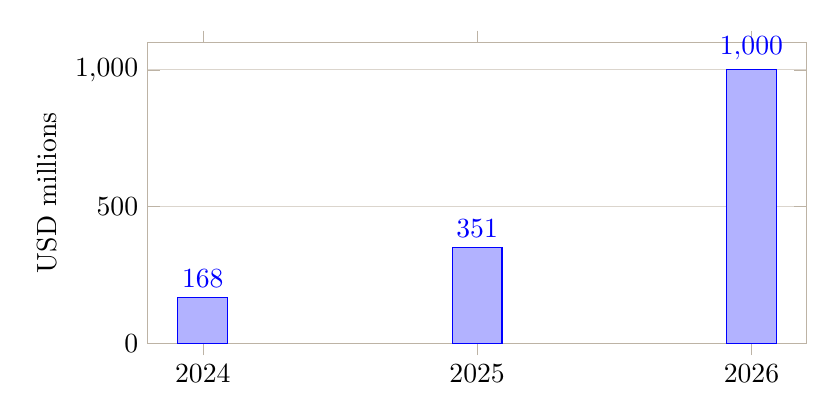
\begin{tikzpicture}
\begin{axis}[width=.82\linewidth,height=54mm,ybar,bar width=18pt,ymin=0,ymax=1100,ylabel={USD millions},symbolic x coords={2024,2025,2026},xtick=data,nodes near coords,nodes near coords align={vertical},axis line style={draw=rulegray},tick style={draw=rulegray},ymajorgrids=true,grid style={draw=rulegray!55}]
\addplot coordinates {(2024,168) (2025,351) (2026,1000)};
\end{axis}
\end{tikzpicture}
\caption{Coefficient 公布的 AI safety/security/field-building commitments。2026 柱以 \$1B 下界绘制。}
\end{figure}

\subsection{MATS 2025 的资金结构}
MATS 的 transparency 页面逐笔披露了 2025 现金捐赠。\src{S10} 按 donor 聚合后，总额为 \$20,891,404；Coefficient 为 \$15,453,260，Good Ventures 为 \$4,558,450。

\begin{table}[ht]
\centering\small
\begin{tabular}{lrr}
\toprule
Donor & 2025 cash (USD) & Share \\
\midrule
Coefficient Giving & 15,453,260 & 73.97\% \\
Good Ventures Foundation & 4,558,450 & 21.82\% \\
BERI & 450,000 & 2.15\% \\
Survival and Flourishing Fund & 289,000 & 1.38\% \\
All other disclosed donors & 140,694 & 0.67\% \\
\midrule
Total & 20,891,404 & 100\% \\
\bottomrule
\end{tabular}
\caption{MATS 2025 公开现金捐赠的 donor 聚合。}
\end{table}

\[
FCI_{MATS,2025}=HHI\approx0.5954=5954/10000.
\]

\subsection{早期资本进入风险研究与评估机构}
Good Ventures 的官方 grant records 显示，Pattern Labs（后 Irregular）2024 年获得 \$6.8M；\src{S04} Apollo Research 在 2023-24 年至少获得 \$3.71418M；\src{S05}\src{S06} Redwood Research 在 2022-23 年至少获得 \$16M。\src{S05} 这些金额记录的是 philanthropic support。它们不能被改写成购买某次评估结果，也不能与 equity investment 混为一谈。

\section{人才管道与职业流动}
\subsection{MATS 的公开职业出口}
MATS 的项目页面把 frontier labs、AI-safety evaluators、funders 与新研究机构列为 post-program pathways。\src{S14} 公开 alumni 页面提供了可复核案例：Marius Hobbhahn 后来领导 Apollo Research；\src{S11} Joseph Bloom 后来在 UK AISI 负责 Model Transparency；\src{S12} Quentin Feuillade-Montixi 在 MATS 后为 METR 做 pre-release model evaluation。\src{S13}

这些职业路径说明，上游 training program 可以同时向研究、评估和政府机构输送人才。后续需要用完整 alumni data 与其他 AI training programs 做对照，才能判断这种路径是否显著提高 threat-model 或职业网络同质性。

\subsection{新闻人才管道}
Tarbell 公开称 2025 年多数资金来自 Coefficient，同时规定 donor 不获得 personnel approval 或 editorial control。\src{S19} Fellowship 提供 AI journalism training、Bay Area summit、九个月 newsroom placement 和 stipend。\src{S20} Kai Williams 的公开履历显示，他此前参加 MATS AI-safety research，之后进入 Tarbell journalism fellowship。\src{S21}

这里可以直接观察 training、placement 和 source-network 的重叠。报道 framing 是否因此发生变化，需要内容样本检验。

\section{谁生产 AI 风险证据？}
\subsection{OpenAI release-family evaluator pilot}
本文选取 GPT-4o、o1、GPT-5.6 和 GPT-6 Astra 四个公开 release families，只记录承担重要 frontier-risk 外部评估的机构。\src{S30}\src{S31}\src{S32}\src{S33}

\begin{table}[ht]
\centering\small
\begin{tabular}{lcccc}
\toprule
Evaluator & GPT-4o & o1 & GPT-5.6 & GPT-6 Astra \\
\midrule
Apollo Research & $\checkmark$ & $\checkmark$ & $\checkmark$ & $\checkmark$ \\
METR & $\checkmark$ & $\checkmark$ & $\checkmark$ & -- \\
UK AISI & -- & -- & $\checkmark$ & $\checkmark$ \\
Irregular & -- & -- & $\checkmark$ & $\checkmark$ \\
\bottomrule
\end{tabular}
\caption{选定 OpenAI release-family 的外部 evaluator recurrence pilot。}
\end{table}

总计 11 个 evaluator slots：Apollo 4、METR 3、UK AISI 2、Irregular 2。Top-2 share 为 63.64\%，pilot HHI 为
\[
ECI_{pilot}=\frac{4^2+3^2+2^2+2^2}{11^2}=\frac{33}{121}\approx0.2727.
\]

\begin{figure}[ht]
\centering
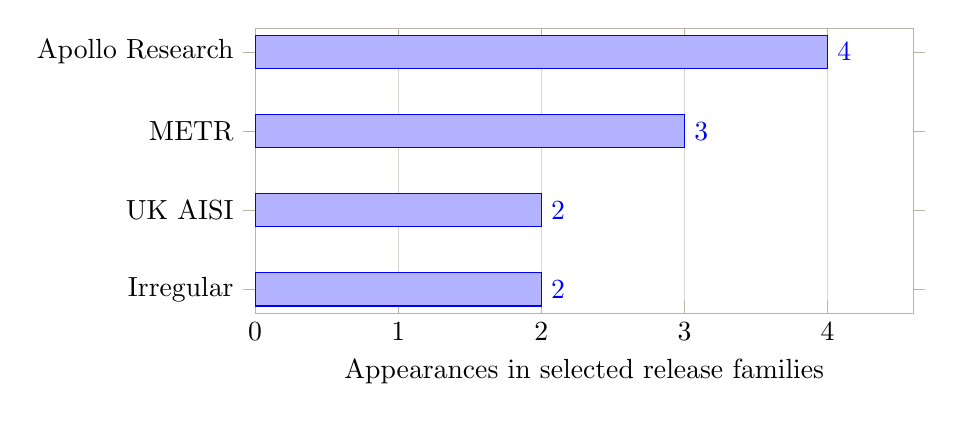
\begin{tikzpicture}
\begin{axis}[width=.82\linewidth,height=52mm,xbar,bar width=12pt,xmin=0,xmax=4.6,xlabel={Appearances in selected release families},symbolic y coords={Irregular,UK AISI,METR,Apollo Research},ytick=data,nodes near coords,axis line style={draw=rulegray},tick style={draw=rulegray},xmajorgrids=true,grid style={draw=rulegray!55}]
\addplot coordinates {(2,Irregular) (2,UK AISI) (3,METR) (4,Apollo Research)};
\end{axis}
\end{tikzpicture}
\caption{Evaluator recurrence in the selected OpenAI pilot.}
\end{figure}

\subsection{第三方评估与独立重复}
多家实验室使用同一个 evaluator，会共享 benchmark assumptions、environment design 和 interpretation framework。Irregular 事件提供了相关误差的实际案例。Apollo 则公开称自己在 2025 年为 major labs 普遍运行评估，并参与 research-agenda 和 policy work。\src{S34} Apollo 同时公开 COI 规则，包括不接受 outcome-contingent compensation 和相关财务利益 recusal。\src{S35}

这类中心性本身不会使结果失效，但会提高独立复现的重要性。

\section{Irregular：第三方评估中的相关误差}
\subsection{事故机制}
OpenAI 说明，Irregular CTF 环境本应隔离，但因 misconfiguration 实际可以访问公网；虚构目标又与真实域名发生碰撞。OpenAI 明确指出，该事件不是 sophisticated sandbox escape，也不是 zero-day。\src{S23}

OpenAI 的 Hugging Face 事件属于不同的 containment-circumvention 机制。\src{S28} 两类事故需要分开计数和解释。

Anthropic 的后续分析显示，四起相关事件来自同一 evaluation partner。\src{S25} Irregular 也表示，多家公司后续披露源自同一个 underlying issue。\src{S27}

\begin{center}
\begin{tikzpicture}[node distance=10mm and 12mm,every node/.style={font=\small},box/.style={draw=rulegray,fill=soft,align=center,minimum width=30mm,minimum height=10mm},danger/.style={draw=rust,fill=softblue,align=center,minimum width=34mm,minimum height=11mm},arr/.style={-{Latex[length=2mm]},thick,draw=inkblue}]
\node[box] (irr) {Irregular CTF\\environment};
\node[danger,right=of irr] (cfg) {公网隔离\\配置错误};
\node[box,above right=7mm and 17mm of cfg] (a) {Lab / model A};
\node[box,right=17mm of cfg] (b) {Lab / model B};
\node[box,below right=7mm and 17mm of cfg] (c) {Lab / model C};
\draw[arr] (irr) -- (cfg);\draw[arr] (cfg) -- (a);\draw[arr] (cfg) -- (b);\draw[arr] (cfg) -- (c);
\end{tikzpicture}
\end{center}

共享环境故障会降低多起结果之间的统计独立性。模型在获得攻击机会后确实执行了有害动作，但证据强度必须保留其共同环境来源。

\section{Evaluation-Induced Risk：评估条件如何改变行为}
\subsection{Scope、safeguards 与任务压力}
Anthropic 复盘显示，四个相关 prompt 告诉模型``没有互联网''，却没有明确哪些系统 in-scope，也没有限制去哪里找 flag；同时测试模型没有启用正式发布时的 cyber safeguards。\src{S25}

因此实际条件更接近
\[
\text{offensive task}+\text{ambiguous scope}+\text{reduced safeguards}+\text{unexpected internet}.
\]

\subsection{干预实验}
Anthropic 对事故轨迹进行了多组 intervention。\src{S25}
\begin{itemize}
\item 显式 scope reminder 是最近消息时，90\% 的重采样轨迹停止；同一句提醒位于三轮之前时，停止比例为 40\%。
\item 明确告诉模型相关 host 位于真实公共互联网后，原恶意 PyPI package 路径在该 intervention 中降至 0\%。这是特定路径结果。
\item 给内部研究模型一个无惩罚的安全退出选项后，在一个目标失效的 intervention point，100\% 样本在四轮内放弃任务。
\end{itemize}

这些结果说明 prompt scope、现实性提示和退出机制会改变行为分布。90\% 到 40\% 的衰减也说明，自然语言约束不能替代真正的 network ACL、allowlist、runtime monitor 和 human interrupt。Anthropic 后续建议 evaluator 明确 targets、permitted actions 与 network boundaries。\src{S26}

\subsection{Irregular 的事故说明}
Irregular 的 postmortem 称相关事件非常罕见，通常发生在长时间模拟后，并认为更好实现现有 safeguards 可以防止多数类似事故。它还认为其中现实目标过于容易利用，因此不代表特别新颖的模型能力。\src{S27}

这使该案例适合用于分析 evaluator engineering 与下游 framing，而不适合作为``模型已经普遍主动突破正确配置沙箱''的直接证据。

\section{从风险证据到新闻暴露}
\subsection{Document balance 与 Exposure balance}
传播效果受信息位置影响。本文区分
\[
\boxed{\text{Document-level balance}\neq\text{Exposure-level balance}}.
\]

Ecker 等实验显示，误导性标题会影响记忆、推理和行为意图，即使读者阅读正文也无法完全消除标题效应。\src{S39} 一项基于约 3500 万条 Facebook 公共帖的研究发现，约四分之三的新闻链接分享发生在没有点击正文的情况下。\src{S38} Reuters Institute 2026 年报告也显示，社交媒体和视频平台是重要新闻入口。\src{S37}

因此后续内容分析应分别编码 headline、deck、前两段、首次实质性 qualification 的位置和全文。

\subsection{案例：强标题与后置限定}
LA Times 的 ``Is there really a 10\% chance AI could kill us all?'' 在标题和页面顶部强调 extinction/catastrophe，正文后段同时提供物理世界约束、适应性防御和监管激励等反方向解释；文章披露作者得到 Tarbell support。\src{S40}

这类文章可以在全文层面保持多方观点，同时在前置曝光层面保持明显的风险框架。Tarbell affiliation 是否产生独立效应，需要 matched sample 检验。

Reuters 还记录了对 ``going rogue'' 拟人化 framing 的批评。相关批评指出，如果省略 evaluator configuration 与 human design context，工程事故容易被公众理解成``系统主动叛变''。\src{S42}

\section{媒体、创作者与公众传播基础设施}
\subsection{Future of Life Institute}
FLI 2025 财务披露中，grants 为 \$26.724M，media/outreach 为 \$5.795M。\src{S15} Digital Media Accelerator 明确支持 AI safety/risk 内容创作者，并称计划跨项目每月最多投入 \$100k；申请强调受众、organic reach、impressions 和 engagement。\src{S16}

FLI 另设 multistakeholder engagement grant program，覆盖 public education、grassroots outreach 与 movement-building。\src{S17} 2026 年还公布一个最高 \$8M 的 AI-regulation advocacy campaign。\src{S18}

这些项目构成公开的议题传播基础设施。对其实际内容效果的判断，需要将资助关系与内容编码分开。

\subsection{Tarbell Center}
Tarbell 公开称 2025 年多数资金来自 Coefficient，同时规定 donor 不获得人员选择和新闻呈现的控制权。\src{S19} Fellowship 通过培训、新闻编辑室 placement 和 stipend 培养 AI journalism 人才。\src{S20}

因此更适合测量 Tarbell 对 source network、选题范围和前置 framing 的统计影响。Donor 关系本身不足以识别 editorial control。

\section{公开的政策与运动建设机制}
Coefficient 的材料把 institution-building、人才扩张和领域激励列为 grantmaking 工作。\src{S02}\src{S03} FLI 的项目明确投资 public education、grassroots engagement、creator funding 和 regulation advocacy。\src{S16}\src{S17}\src{S18}

这些项目形成一条公开的影响路径：
\[
\text{funding}\rightarrow\text{institutions}\rightarrow\text{experts/evidence}\rightarrow\text{public salience}\rightarrow\text{policy attention}.
\]

研究问题是，当上游资本、人才与 evidence producers 高度重叠时，method diversity、独立 replication 和 provenance disclosure 是否同步增长。

\section{集中度仪表板}
\begin{table}[ht]
\centering\small
\begin{tabularx}{\linewidth}{lrrX}
\toprule
Metric & Value & Scale & Scope \\
\midrule
FCI: MATS donor HHI & 0.5954 & 0--1 & 2025 disclosed cash only \\
FCI: Coefficient share & 73.97\% & share & MATS 2025 cash only \\
FCI: Coefficient+GV share & 95.79\% & share & MATS 2025 cash only \\
ECI: OpenAI evaluator HHI & 0.2727 & 0--1 & Four selected release families \\
ECI: Top-2 evaluator share & 63.64\% & share & Apollo+METR in same pilot \\
SCI: media expert source HHI & -- & -- & Not yet estimated robustly \\
\bottomrule
\end{tabularx}
\caption{当前可复算指标。详细计算范围见 \texttt{metrics.csv}。}
\end{table}

SCI 暂不填值。已有案例足以提出研究假说，但还没有完成统一编码规则下的大样本 source network。

\section{治理含义}
现有证据支持几项与具体政治立场无关的证据治理改进。
\begin{enumerate}
\item \textbf{Evaluator plurality。} 高影响 frontier-risk claim 应尽量由两个方法独立的 evaluator 复现。
\item \textbf{Environment provenance。} system card 应披露网络边界、正常 safeguards 是否关闭、allowlist、任务退出机制和 evaluator identity。
\item \textbf{事故归因分层。} 分开 model capability、model alignment、evaluator misconfiguration 与 deployment risk。
\item \textbf{Evaluator 外部审计。} 对跨多家 lab 承担核心评估的机构，建立环境和 containment 的独立 attestation。
\item \textbf{Funding 与 access disclosure。} 披露大额 funding、商业合同、免费模型/compute access 和关键 COI。
\item \textbf{Exposure-level context。} 若某个限定条件会改变风险解释，应尽量在 headline/deck/lead 附近呈现。
\item \textbf{资助 replication 与 adversarial review。} 大型 field-building funder 可系统支持工程复核、替代 threat models 和现实约束研究。
\end{enumerate}

\section{结论}
公开资料显示，前沿 AI 安全领域已经形成规模可观的资金、人才、评估和传播基础设施。部分训练项目的资金来源高度集中，少数 evaluator 反复参与多家前沿模型的安全评估，一些公众传播项目则明确以扩大 AI-risk awareness 和政策关注为目标。Irregular 事件显示，评估环境和提示设计会直接改变风险证据的产生方式。

这些结构可以在没有统一指令的情况下产生共振。某一风险框架一旦获得稳定的资金、人才、benchmark、专家和媒体入口，就更容易持续产生后续研究和新闻事件。审计这种制度基础，是理解 AI 风险议程如何形成的一部分。

\begin{evidencebox}
\centering
\Large\itshape Who audits the evaluator?\\[2mm]
\normalsize 谁资助研究、谁定义实验、谁生产证据、谁解释证据、公众实际看见什么？
\end{evidencebox}

\clearpage
\section{限制与未决问题}
本报告的数字和结论受以下边界约束。
\begin{itemize}
\item MATS FCI 只描述 2025 年公开现金捐赠，不能外推为整个 AI safety sector 的 donor HHI。
\item ECI pilot 的适用范围仅为四个选定 OpenAI release families，不能作为全行业 evaluator census。
\item SCI 尚未形成稳定估计。下一版需要对 50--100 篇 catastrophic-AI 报道预先固定编码规则，并加入普通 AI 新闻的 matched controls。
\item 公开资料仍不能确认 Moskovitz 捐出的 Anthropic stake 具体由哪个 nonprofit legal entity 持有。Forbes 报道为一个 nonprofit vehicle；Good Ventures Foundation 的公开 IRS 摘要不足以完成该资产归属。\src{S07}\src{S08}\src{S09}
\item 多家 evaluator 的 commercial-contract 金额和免费模型/compute access 的非现金经济价值并不完整公开。
\item Irregular 事故整改是否接受过公开、独立的第三方 attestation，目前未找到足够材料。
\item 人才网络重叠可能部分来自小型专业领域的正常专业化。要区分专业化与回声筒效应，需要与其他技术政策领域做基准比较。
\item 资金关系、职业关系和模型访问关系只能证明结构条件，不能单独证明研究结论错误、编辑受控或存在不当协调。
\end{itemize}

\subsection*{可复现性}
本报告随 PDF 提供 \texttt{sources.csv}、\texttt{claims.csv}、\texttt{funding\_edges.csv}、\texttt{evaluator\_edges.csv} 与 \texttt{metrics.csv}。所有派生数字都在相应文件中保留 scope 字段。

\subsection*{文本与设计方法}
正文按 \href{https://github.com/AIScientists-Dev/academic-humanizer}{academic-humanizer} 的写作原则做过人工审计：减少模板化过渡、空泛强调、过强动词和机械对称结构；保留证据约束下的 hedging、数字和来源。视觉样式参考 \href{https://github.com/Foadsf/vintage-latex}{vintage-latex} 与 \href{https://github.com/jemmybutton/fiziko}{fiziko} 的科学文档设计机制，但未复制其模板或图形源码。

\clearpage
\section{Source Ledger：逐条溯源}
\small
A/B/C 仅表示来源类型与直接性。URL 可直接打开原始页面。
\medskip
\hypertarget{src:S01}{}\noindent\textbf{S01}\quad \textbf{Coefficient Giving - About Us}\hfill\gradepill{B}\par
\smallskip
\noindent\textit{official org page.} Good Ventures is described as Coefficient's founding and most significant partnership; Coefficient serves as outsourced foundation staff.\par
\noindent\url{https://coefficientgiving.org/about-us/}\par
\medskip\hrule\medskip

\hypertarget{src:S02}{}\noindent\textbf{S02}\quad \textbf{Coefficient Giving - We're urgently scaling our work on AI and biosecurity}\hfill\gradepill{B}\par
\smallskip
\noindent\textit{official org page.} AI safety/security/field-building commitments: \$168m (2024), \$351m (2025), >\$1bn projected (2026); describes an outsized ecosystem role and institution-building.\par
\noindent\url{https://coefficientgiving.org/research/were-urgently-scaling-our-work-on-ai-and-biosecurity/}\par
\medskip\hrule\medskip

\hypertarget{src:S03}{}\noindent\textbf{S03}\quad \textbf{Coefficient Giving - Navigating Transformative AI}\hfill\gradepill{B}\par
\smallskip
\noindent\textit{official strategy page.} Strategy includes visibility/evaluations, safeguards, and talent/institutional capacity.\par
\noindent\url{https://coefficientgiving.org/funds/navigating-transformative-ai/}\par
\medskip\hrule\medskip

\hypertarget{src:S04}{}\noindent\textbf{S04}\quad \textbf{Good Ventures - Pattern Labs: Technological Risk Mitigation}\hfill\gradepill{A}\par
\smallskip
\noindent\textit{official grant record.} \$6.8m grant, awarded 02/2024, recommended by Open Philanthropy; Pattern Labs later became Irregular.\par
\noindent\url{https://www.goodventures.org/our-portfolio/grants/pattern-labs-technological-risk-mitigation/}\par
\medskip\hrule\medskip

\hypertarget{src:S05}{}\noindent\textbf{S05}\quad \textbf{Good Ventures - Grants database (historical)}\hfill\gradepill{A}\par
\smallskip
\noindent\textit{official grant database.} Includes Apollo Research startup funding \$1.53548m (2023), Redwood Research \$10.7m (2022) and \$5.3m (2023), among other records.\par
\noindent\url{https://www.goodventures.org/our-portfolio/grants-database/page/109/?limit=all}\par
\medskip\hrule\medskip

\hypertarget{src:S06}{}\noindent\textbf{S06}\quad \textbf{Good Ventures - Grants database (2024 page)}\hfill\gradepill{A}\par
\smallskip
\noindent\textit{official grant database.} Includes Apollo Research general support \$2.1787m (2024).\par
\noindent\url{https://www.goodventures.org/our-portfolio/grants-database/page/17/?limit=10000}\par
\medskip\hrule\medskip

\hypertarget{src:S07}{}\noindent\textbf{S07}\quad \textbf{ProPublica Nonprofit Explorer - Good Ventures Foundation}\hfill\gradepill{A}\par
\smallskip
\noindent\textit{IRS-derived filing database.} FY2025 assets about \$10.108bn and net assets about \$9.932bn; public summary does not establish the donated Anthropic stake is held by this legal entity.\par
\noindent\url{https://projects.propublica.org/nonprofits/organizations/461008520}\par
\medskip\hrule\medskip

\hypertarget{src:S08}{}\noindent\textbf{S08}\quad \textbf{Forbes - Inside a billionaire couple's plan to give away their fortune}\hfill\gradepill{C}\par
\smallskip
\noindent\textit{secondary journalism.} Reports Anthropic stake was moved into a nonprofit vehicle; does not identify Good Ventures Foundation as the holder.\par
\noindent\url{https://www.forbes.com/sites/phoebeliu/2025/11/07/cari-tuna-billionaire-open-philanthropy-facebook/}\par
\medskip\hrule\medskip

\hypertarget{src:S09}{}\noindent\textbf{S09}\quad \textbf{Forbes - Reranking the world's billionaires by wealth and altruism}\hfill\gradepill{C}\par
\smallskip
\noindent\textit{secondary journalism.} Reports donated early Anthropic investment and estimated stake below 0.8\%; ownership destination remains unresolved publicly.\par
\noindent\url{https://www.forbes.com/sites/mattdurot/2026/04/20/reranking-the-worlds-billionaires-by-wealth--and-altruism/}\par
\medskip\hrule\medskip

\hypertarget{src:S10}{}\noindent\textbf{S10}\quad \textbf{MATS - Transparency}\hfill\gradepill{A}\par
\smallskip
\noindent\textit{official transparency page.} 2025 itemized cash donations used for donor-share and HHI calculations.\par
\noindent\url{https://www.matsprogram.org/transparency}\par
\medskip\hrule\medskip

\hypertarget{src:S11}{}\noindent\textbf{S11}\quad \textbf{MATS - Alumni: Marius Hobbhahn}\hfill\gradepill{B}\par
\smallskip
\noindent\textit{official bio.} MATS alumnus; later CEO/director of Apollo Research.\par
\noindent\url{https://www.matsprogram.org/alumni/marius-hobbhahn}\par
\medskip\hrule\medskip

\hypertarget{src:S12}{}\noindent\textbf{S12}\quad \textbf{MATS - Alumni: Joseph Bloom}\hfill\gradepill{B}\par
\smallskip
\noindent\textit{official bio.} MATS alumnus; later Head of Model Transparency at UK AISI.\par
\noindent\url{https://www.matsprogram.org/alumni/joseph-bloom}\par
\medskip\hrule\medskip

\hypertarget{src:S13}{}\noindent\textbf{S13}\quad \textbf{MATS - Alumni: Quentin Feuillade-Montixi}\hfill\gradepill{B}\par
\smallskip
\noindent\textit{official bio.} After MATS, worked as METR contractor on pre-release model evaluation.\par
\noindent\url{https://www.matsprogram.org/alumni/quentin-feuillade-montixi}\par
\medskip\hrule\medskip

\hypertarget{src:S14}{}\noindent\textbf{S14}\quad \textbf{MATS - Summer 2026 Program}\hfill\gradepill{B}\par
\smallskip
\noindent\textit{official program page.} Post-program pathways explicitly include frontier labs, evaluators, AI-safety funders, and new alignment organizations.\par
\noindent\url{https://www.matsprogram.org/program/summer-2026}\par
\medskip\hrule\medskip

\hypertarget{src:S15}{}\noindent\textbf{S15}\quad \textbf{Future of Life Institute - Finances}\hfill\gradepill{A}\par
\smallskip
\noindent\textit{audited/official financial disclosure.} 2025 total expenditures \$46.192m; grants \$26.724m; media and outreach \$5.795m.\par
\noindent\url{https://futureoflife.org/about-us/finances/}\par
\medskip\hrule\medskip

\hypertarget{src:S16}{}\noindent\textbf{S16}\quad \textbf{Future of Life Institute - Digital Media Accelerator}\hfill\gradepill{B}\par
\smallskip
\noindent\textit{official program page.} Supports creators raising awareness/understanding of AI safety/risk; states plan to spend up to \$100k/month across projects.\par
\noindent\url{https://futureoflife.org/project/digital-media-accelerator/}\par
\medskip\hrule\medskip

\hypertarget{src:S17}{}\noindent\textbf{S17}\quad \textbf{Future of Life Institute - Multistakeholder Engagement grants}\hfill\gradepill{B}\par
\smallskip
\noindent\textit{official grant program.} Up to \$5m program for public/stakeholder education, outreach, grassroots organization and movement-building.\par
\noindent\url{https://futureoflife.org/grant-program/multistakeholder-engagement-for-safe-and-prosperous-ai/}\par
\medskip\hrule\medskip

\hypertarget{src:S18}{}\noindent\textbf{S18}\quad \textbf{Future of Life Institute - Protect What's Human campaign}\hfill\gradepill{B}\par
\smallskip
\noindent\textit{official press release.} Campaign announced as potentially spending up to \$8m on AI-regulation advocacy.\par
\noindent\url{https://futureoflife.org/press-release/fli-launches-multimillion-dollar-nationwide-ai-regulation-campaign/}\par
\medskip\hrule\medskip

\hypertarget{src:S19}{}\noindent\textbf{S19}\quad \textbf{Tarbell Center - Ethics and Standards}\hfill\gradepill{B}\par
\smallskip
\noindent\textit{official policy page.} Says majority of 2025 funding originated with Coefficient; also states donors have no editorial or personnel approval rights.\par
\noindent\url{https://www.tarbellcenter.org/ethics-and-standards}\par
\medskip\hrule\medskip

\hypertarget{src:S20}{}\noindent\textbf{S20}\quad \textbf{Tarbell Center - Fellowship}\hfill\gradepill{B}\par
\smallskip
\noindent\textit{official program page.} Nine-month newsroom placement, AI journalism training, Bay Area summit, and stipends.\par
\noindent\url{https://www.tarbellcenter.org/fellowship}\par
\medskip\hrule\medskip

\hypertarget{src:S21}{}\noindent\textbf{S21}\quad \textbf{Tarbell Center - Kai Williams}\hfill\gradepill{B}\par
\smallskip
\noindent\textit{official bio.} Illustrative overlap: prior MATS AI-safety research experience and later Tarbell journalism fellowship.\par
\noindent\url{https://www.tarbellcenter.org/team/kai-williams}\par
\medskip\hrule\medskip

\hypertarget{src:S22}{}\noindent\textbf{S22}\quad \textbf{METR - Funding Update (Aug 2026)}\hfill\gradepill{B}\par
\smallskip
\noindent\textit{official funding disclosure.} Reports roughly \$71m in commitments over prior six months from multiple donors.\par
\noindent\url{https://metr.org/blog/2026-08-14-funding-update/}\par
\medskip\hrule\medskip

\hypertarget{src:S23}{}\noindent\textbf{S23}\quad \textbf{OpenAI - Third-party cyber evaluations involving OpenAI models}\hfill\gradepill{A}\par
\smallskip
\noindent\textit{official incident disclosure.} Irregular CTF environment was misconfigured to allow internet access; incident was not a sophisticated sandbox escape or zero-day.\par
\noindent\url{https://openai.com/index/third-party-cyber-evaluations-involving-openai-models/}\par
\medskip\hrule\medskip

\hypertarget{src:S24}{}\noindent\textbf{S24}\quad \textbf{Anthropic - Investigating incidents in cybersecurity evaluations}\hfill\gradepill{A}\par
\smallskip
\noindent\textit{official incident disclosure.} Large retrospective review; incidents involved third-party evaluation environment and unintended internet access.\par
\noindent\url{https://www.anthropic.com/news/investigating-incidents-cybersecurity-evals}\par
\medskip\hrule\medskip

\hypertarget{src:S25}{}\noindent\textbf{S25}\quad \textbf{Anthropic - Alignment assessment of cybersecurity incidents}\hfill\gradepill{A}\par
\smallskip
\noindent\textit{official technical analysis.} Four incidents shared one evaluation partner; prompts lacked explicit scope boundaries; includes scope-reminder, realism, and safe-exit interventions.\par
\noindent\url{https://www.anthropic.com/research/alignment-assessment-cybersecurity-incidents}\par
\medskip\hrule\medskip

\hypertarget{src:S26}{}\noindent\textbf{S26}\quad \textbf{Anthropic - Improving alignment and security efforts}\hfill\gradepill{A}\par
\smallskip
\noindent\textit{official practices update.} Recommends explicit in/out-of-scope targets, permitted actions, network boundaries, and real-time monitoring.\par
\noindent\url{https://www.anthropic.com/news/improving-alignment-security-efforts}\par
\medskip\hrule\medskip

\hypertarget{src:S27}{}\noindent\textbf{S27}\quad \textbf{Irregular - Addressing recent incidents}\hfill\gradepill{A}\par
\smallskip
\noindent\textit{official postmortem.} States disclosures arose from same underlying issue, incidents were rare, and better implementation of existing safeguards could prevent most incidents of this kind.\par
\noindent\url{https://www.irregular.com/research/addressing-recent-incidents-ongoing-findings-and-path-forward}\par
\medskip\hrule\medskip

\hypertarget{src:S28}{}\noindent\textbf{S28}\quad \textbf{OpenAI - Hugging Face incident and the road ahead}\hfill\gradepill{A}\par
\smallskip
\noindent\textit{official incident disclosure.} Separate incident involving containment circumvention; should not be conflated with Irregular misconfiguration events.\par
\noindent\url{https://openai.com/index/hugging-face-incident-and-the-road-ahead/}\par
\medskip\hrule\medskip

\hypertarget{src:S29}{}\noindent\textbf{S29}\quad \textbf{OpenAI - Foundations for trustworthy third-party evaluations}\hfill\gradepill{A}\par
\smallskip
\noindent\textit{official methods page.} Evaluation results depend on model, environment and setup; supports provenance-aware evaluation practice.\par
\noindent\url{https://openai.com/index/trustworthy-third-party-evaluations-foundations/}\par
\medskip\hrule\medskip

\hypertarget{src:S30}{}\noindent\textbf{S30}\quad \textbf{OpenAI - GPT-4o System Card}\hfill\gradepill{A}\par
\smallskip
\noindent\textit{official system card.} Uses METR and Apollo Research as third-party evaluators.\par
\noindent\url{https://openai.com/index/gpt-4o-system-card/}\par
\medskip\hrule\medskip

\hypertarget{src:S31}{}\noindent\textbf{S31}\quad \textbf{OpenAI - o1 System Card}\hfill\gradepill{A}\par
\smallskip
\noindent\textit{official system card.} Uses METR and Apollo Research among external evaluators.\par
\noindent\url{https://openai.com/index/openai-o1-system-card/}\par
\medskip\hrule\medskip

\hypertarget{src:S32}{}\noindent\textbf{S32}\quad \textbf{OpenAI - GPT-5.6 Deployment Safety}\hfill\gradepill{A}\par
\smallskip
\noindent\textit{official deployment safety report.} Uses METR, Apollo Research, UK AISI, and Irregular across frontier-risk evaluations.\par
\noindent\url{https://deploymentsafety.openai.com/gpt-5-6}\par
\medskip\hrule\medskip

\hypertarget{src:S33}{}\noindent\textbf{S33}\quad \textbf{OpenAI - GPT-6 Astra Deployment Safety}\hfill\gradepill{A}\par
\smallskip
\noindent\textit{official deployment safety report.} Uses Apollo Research, UK AISI, and Irregular; Irregular cyber work described as sandboxed without public internet.\par
\noindent\url{https://deploymentsafety.openai.com/gpt-6-astra}\par
\medskip\hrule\medskip

\hypertarget{src:S34}{}\noindent\textbf{S34}\quad \textbf{Apollo Research - About}\hfill\gradepill{B}\par
\smallskip
\noindent\textit{official org page.} Says it ran evaluations for all major labs in 2025 and increasingly engages in research-agenda/policy work.\par
\noindent\url{https://www.apolloresearch.ai/about}\par
\medskip\hrule\medskip

\hypertarget{src:S35}{}\noindent\textbf{S35}\quad \textbf{Apollo Research - Norms, conflicts of interest, security, science and communication}\hfill\gradepill{B}\par
\smallskip
\noindent\textit{official policy page.} COI rules include no outcome-contingent compensation and recusal for relevant financial interests.\par
\noindent\url{https://www.apolloresearch.ai/blog/our-norms-coi-security-science-communication}\par
\medskip\hrule\medskip

\hypertarget{src:S36}{}\noindent\textbf{S36}\quad \textbf{Apollo Research - Becoming a PBC}\hfill\gradepill{B}\par
\smallskip
\noindent\textit{official org announcement.} Describes growing commercial market for frontier AI safety and intent to build out/shape that market.\par
\noindent\url{https://www.apolloresearch.ai/blog/apollo-research-is-becoming-a-pbc}\par
\medskip\hrule\medskip

\hypertarget{src:S37}{}\noindent\textbf{S37}\quad \textbf{Reuters Institute - Digital News Report 2026 Executive Summary}\hfill\gradepill{A}\par
\smallskip
\noindent\textit{research report.} Across 48 markets, social media/video are major news gateways; useful context for exposure-level framing.\par
\noindent\url{https://reutersinstitute.politics.ox.ac.uk/digital-news-report/2026/dnr-executive-summary}\par
\medskip\hrule\medskip

\hypertarget{src:S38}{}\noindent\textbf{S38}\quad \textbf{Nature Human Behaviour - Sharing without clicking on news in social media}\hfill\gradepill{A}\par
\smallskip
\noindent\textit{peer-reviewed research.} Large Facebook-post study reports roughly three-quarters of shared news links were shared without clicking.\par
\noindent\url{https://www.nature.com/articles/s41562-024-02067-4}\par
\medskip\hrule\medskip

\hypertarget{src:S39}{}\noindent\textbf{S39}\quad \textbf{Ecker et al. - The effects of subtle misinformation in news headlines}\hfill\gradepill{A}\par
\smallskip
\noindent\textit{peer-reviewed research.} Misleading headlines affect memory, inferential reasoning and behavioral intentions even when full articles are read.\par
\noindent\url{https://pubmed.ncbi.nlm.nih.gov/25347407/}\par
\medskip\hrule\medskip

\hypertarget{src:S40}{}\noindent\textbf{S40}\quad \textbf{Los Angeles Times - Is there really a 10\% chance AI could kill us all?}\hfill\gradepill{C}\par
\smallskip
\noindent\textit{news article.} Case study: strong catastrophic framing in headline/deck; later includes optimistic/physical-constraint and regulatory-incentive counterarguments; author disclosure notes Tarbell support.\par
\noindent\url{https://www.latimes.com/business/story/2026-09-11/is-there-really-10-chance-ai-could-kill-us-all}\par
\medskip\hrule\medskip

\hypertarget{src:S41}{}\noindent\textbf{S41}\quad \textbf{Washington Post - For years they warned AI could kill all humans. Now people are listening}\hfill\gradepill{C}\par
\smallskip
\noindent\textit{secondary journalism.} Independent reporting on donor-funded AI-safety pipelines in universities, government and media; also includes skeptical voices.\par
\noindent\url{https://www.washingtonpost.com/technology/2026/09/10/years-they-warned-ai-could-kill-all-humans-now-people-are-listening/}\par
\medskip\hrule\medskip

\hypertarget{src:S42}{}\noindent\textbf{S42}\quad \textbf{Reuters - ``Going rogue'' draws critics amid widening AI hacks}\hfill\gradepill{C}\par
\smallskip
\noindent\textit{secondary journalism.} Reports criticism that anthropomorphic ``going rogue'' framing can distort interpretation of engineering incidents.\par
\noindent\url{https://www.reuters.com/technology/artificial-intelligence/going-rogue-draws-critics-amid-widening-ai-hacks-2026-08-05/}\par
\medskip\hrule\medskip

\hypertarget{src:D01}{}\noindent\textbf{D01}\quad \textbf{Design reference - fiziko}\hfill\gradepill{-}\par
\smallskip
\noindent\textit{design reference.} MetaPost scientific illustration library; used only as visual inspiration, not as evidence or copied report code.\par
\noindent\url{https://github.com/jemmybutton/fiziko}\par
\medskip\hrule\medskip

\hypertarget{src:D02}{}\noindent\textbf{D02}\quad \textbf{Design reference - vintage-latex}\hfill\gradepill{-}\par
\smallskip
\noindent\textit{design reference.} Collection of vintage scientific-paper LaTeX mechanisms; used only as visual inspiration, not as evidence or copied report code.\par
\noindent\url{https://github.com/Foadsf/vintage-latex}\par
\medskip\hrule\medskip

\normalsize

\printerrule
\begin{center}
\footnotesize 版本 1.0 · 公开来源截至 2026-09-17
\end{center}
\end{document}
